\documentclass[a4paper]{article}
\usepackage[T1]{fontenc}			% pacchetto per \chapter
\usepackage[italian]{babel}
\usepackage[italian]{isodate}  		% formato delle date in italiano
\usepackage{lipsum}
\usepackage{graphicx}				% gestione delle immagini
\usepackage{amsfonts}
\usepackage{booktabs}				% tabelle di qualità superiore
\usepackage{amsmath}				% pacchetto matematica
\usepackage{amsthm}					% teoremi migliorati
\usepackage{enumitem}				% gestione delle liste
\usepackage{pifont}					% pacchetto con elenchi carini
\usepackage{listings}				% pacchetto per i codici
\usepackage{caption}
\usepackage{cancel}
\usepackage[x11names]{xcolor}		% pacchetto colori RGB
% Link ipertestuali per l'indice
\usepackage{xcolor}
\usepackage[linkcolor=black, citecolor=blue, urlcolor=cyan]{hyperref}
\hypersetup{
	colorlinks=true
}

\definecolor{codegreen}{rgb}{0,0.6,0}
\definecolor{codegray}{rgb}{0.5,0.5,0.5}
\definecolor{codepurple}{rgb}{0.58,0,0.82}
\definecolor{backcolour}{rgb}{0.95,0.95,0.92}
\lstdefinestyle{mystyle}{
	backgroundcolor=\color{backcolour},   
	commentstyle=\color{codegreen},
	keywordstyle=\color{magenta},
	numberstyle=\tiny\color{codegray},
	stringstyle=\color{codepurple},
	basicstyle=\ttfamily\footnotesize,
	breakatwhitespace=false,         
	breaklines=true,                 
	captionpos=b,                    
	keepspaces=true,                 
	numbers=left,                    
	numbersep=5pt,                  
	showspaces=false,                
	showstringspaces=false,
	showtabs=false,                  
	tabsize=2
}
\lstset{style=mystyle}

%\usepackage{showframe}				% visualizzazione bordi
%\usepackage{showkeys}				% visualizzazione etichetta

\newcommand{\longline}{\noindent\rule{\textwidth}{0.4pt}}
\newcommand{\dquotes}[1]{``#1''}
\renewcommand{\qedsymbol}{QED}

\begin{document}
	\author{VR443470}
	\title{Esami - Basi di dati}
	\date{\printdayoff\today}
	\maketitle

	\newpage
	
	% indice
	\tableofcontents
	
	\newpage
		
	\section{Domande di teoria - Primo parziale}
	
	Le domande più frequenti che si possono incontrare nel primo parziale di Basi di dati sono:
	\begin{enumerate}
		\item Si illustri il concetto/costrutto di \textbf{entità} nel modello Entità-Relazione.
		
		\item Si illustri il concetto/costrutto di \textbf{relazione} nel modello Entità-Relazione.
		
		\item Si illustri il concetto/costrutto di \textbf{generalizzazione} nel modello Entità-Relazione.
		
		\item Si illustri il concetto/costrutto di \textbf{identificatore} nel modello Entità-Relazione.
		
		\item Si illustri il concetto/costrutto di \textbf{superchiave} nel modello Entità-Relazione.
		
		\item Si illustri il concetto/costrutto di \textbf{attributo multivalore} nel modello Entità-Relazione.
	\end{enumerate}
	La risposta, per essere considerata perfetta, deve includere le seguenti caratteristiche:
	\begin{itemize}
		\item Semantica
		\item Sintassi grafica con esempio
		\item Istanza
		\item Eventuali proprietà
	\end{itemize}
	Qui di seguito vengono date le possibili risposte alle domande di teoria:
	\begin{enumerate}
		\item \textcolor{Green4}{\emph{Si illustri il concetto/costrutto di \textbf{entità} nel modello Entità-Relazione.}}
		
		\textbf{Semantica}. L'entità rappresenta una classe di oggetti che hanno proprietà comuni ed esistenza \dquotes{autonoma} ai fini dell'applicazione di interesse. Il nome dato ad ogni entità è identificativo di quella determinata classe di oggetti e deve essere univoco all'interno dello schema.\newline
		\textbf{Sintassi grafica}. Per esempio, l'entità studenti rappresenta la classe di oggetti degli studenti di un'università e gli attributi possibili possono essere: matricola, nome, cognome, data di nascita, ecc. La sintassi grafica è la seguente:
		\begin{figure}[!htp]
			\centering
			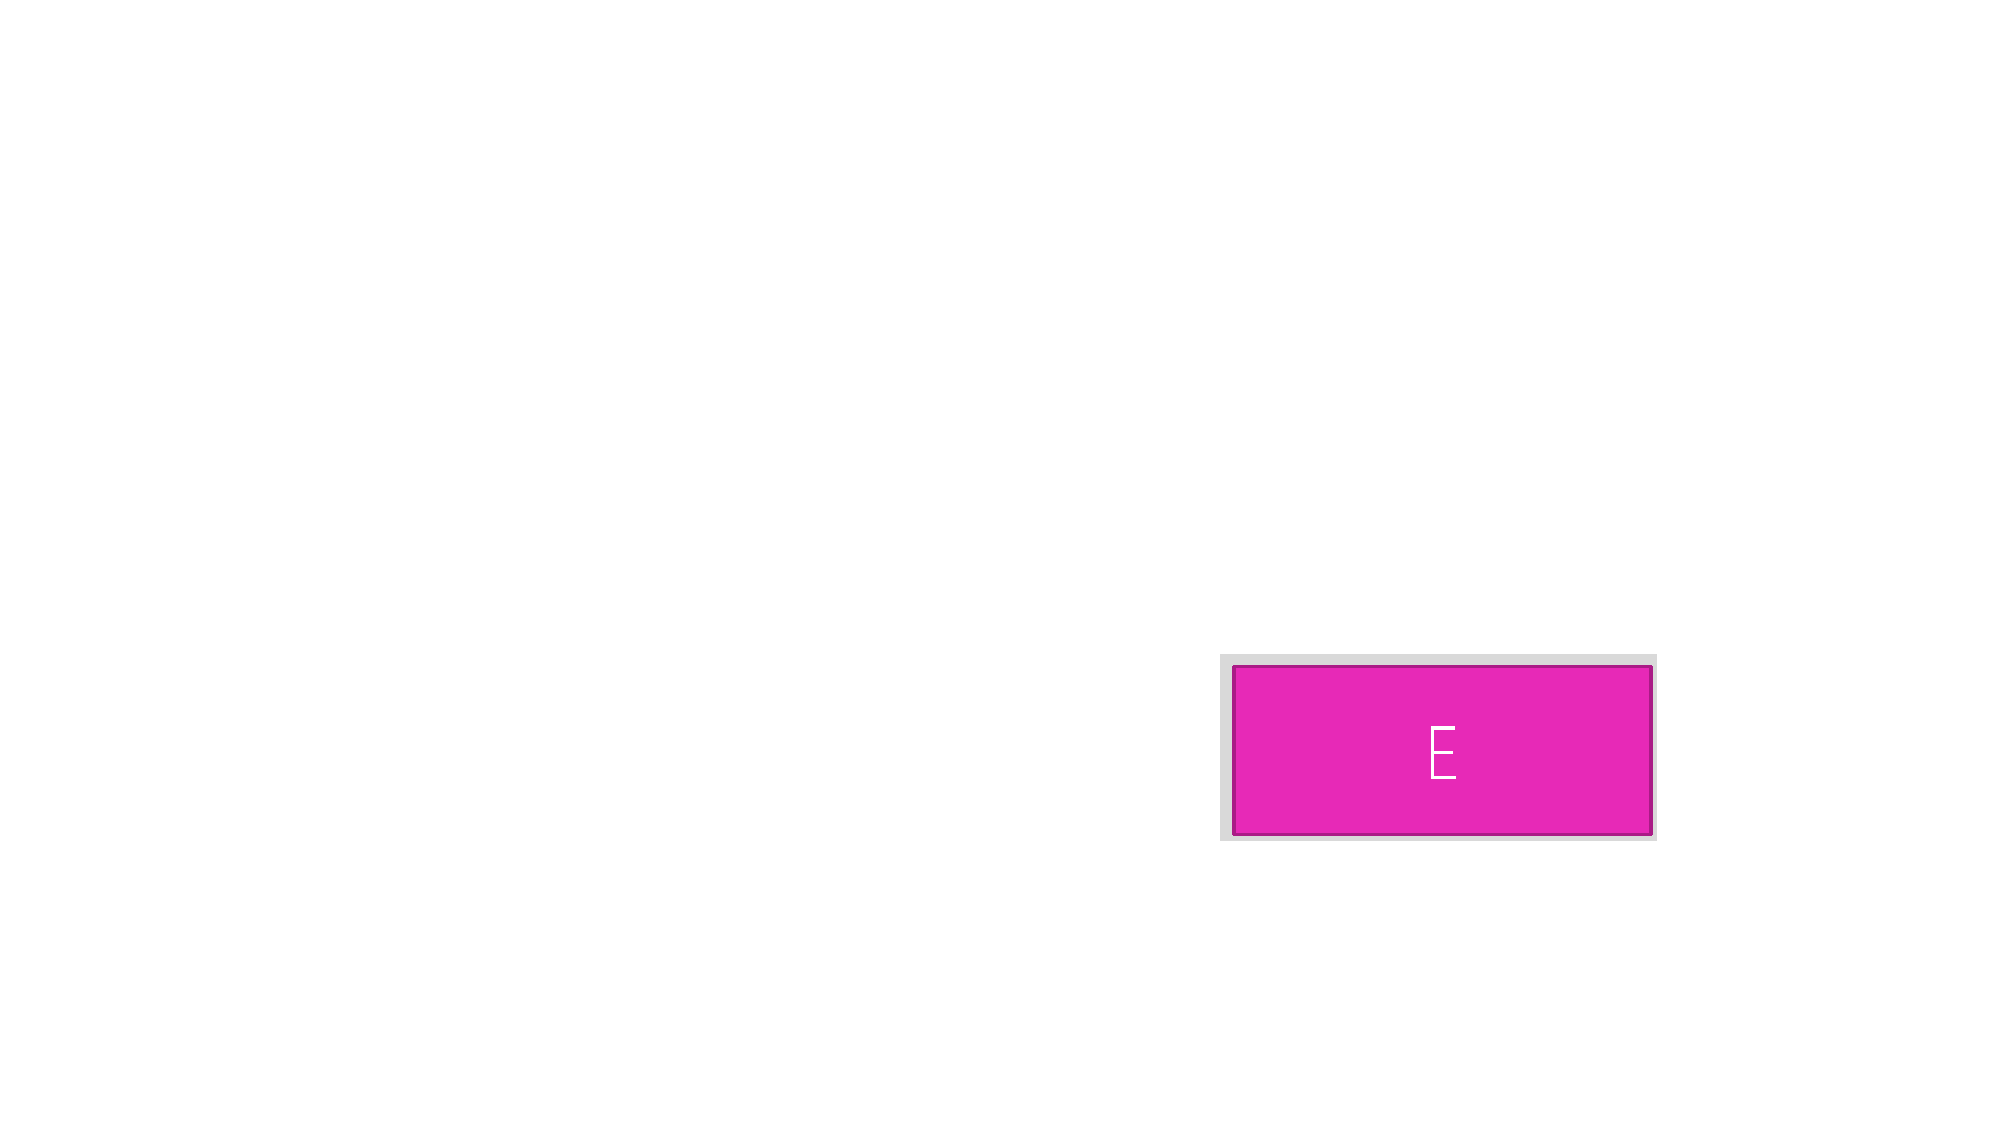
\includegraphics[width=.3\textwidth]{img/entita_def.pdf}
		\end{figure}
		
		\noindent
		\textbf{Istanza}. L'istanza di un'entità è un oggetto della classe che lo rappresenta e non un unico valore. Per esempio, nell'entità studenti, lo studente Mario Rossi (in carne ed ossa) rappresenta un'istanza dell'entità.
		\newpage
		
		
		\item \textcolor{Green4}{\emph{Si illustri il concetto/costrutto di \textbf{relazione} nel modello Entità-Relazione.}}
		
		\textbf{Semantica}. La relazione rappresenta legami logici tra una o più entità. Ogni relazione deve avere un nome univoco all'interno dello schema e non può avere identificatori. Esistono due tipi di relazioni: \emph{ricorsive}, cioè in cui è coinvolta una sola entità, \emph{n-arie}, in cui sono coinvolte \emph{n} entità. Esse nascono solo quando le entità coinvolte contengono almeno una tupla.\newline
		\textbf{Sintassi grafica}. Un esempio di relazione è la \dquotes{Residenza} tra le entità \dquotes{Città} e \dquotes{Impiegato}. La sua sintassi grafica è un rombo:
		\begin{figure}[!htp]
			\centering
			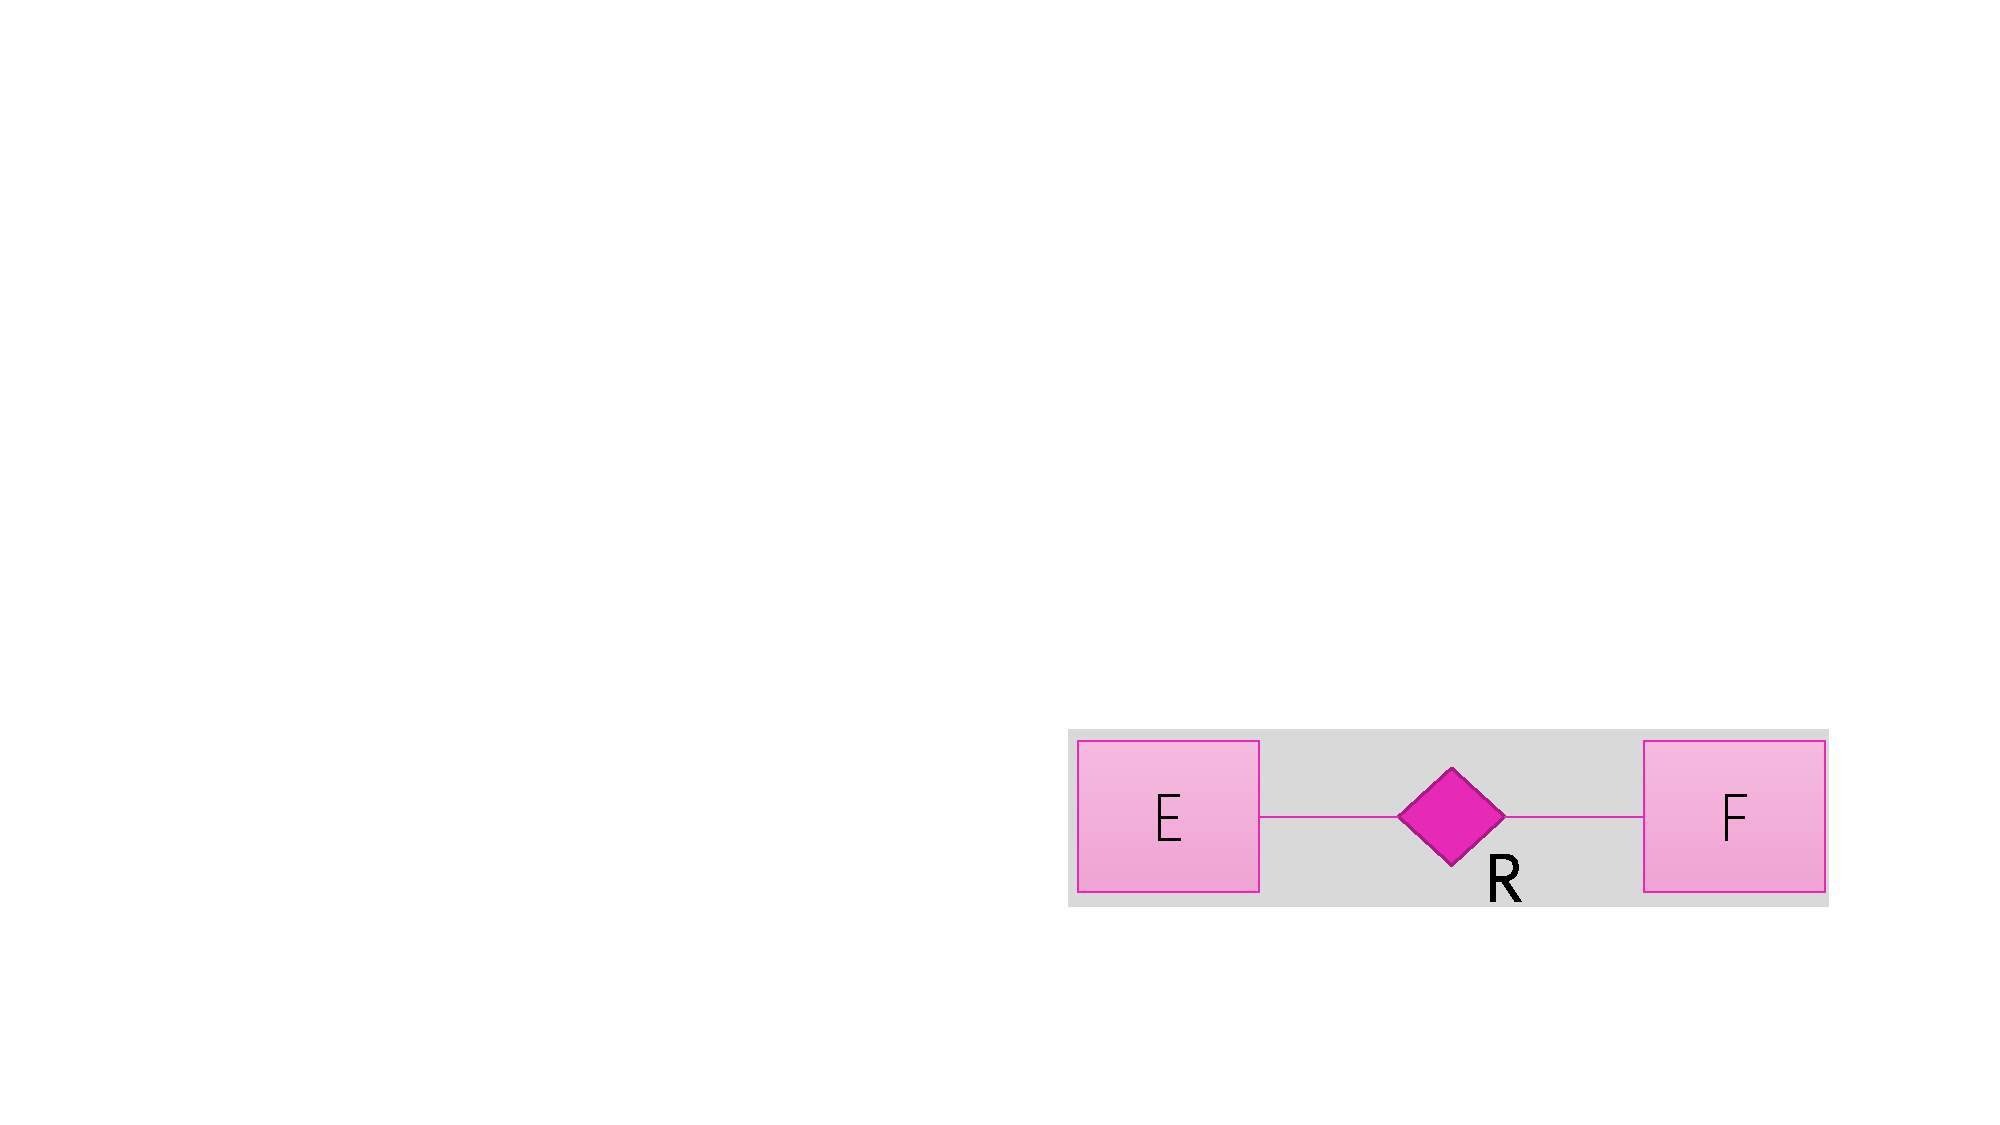
\includegraphics[width=.5\textwidth]{img/relazione_def.pdf}
		\end{figure}
		
		\noindent
		\textbf{Istanza}. Data una relazione $R$ tra $n$ entità $E_{1}, E_{2}, ..., E_{n}$, un'istanza è composta da una ennupla del tipo:
		\begin{equation*}
			\left(e_{1}, e_{2}, ..., e_{i}\right) \: \text{dove} \: e_{i} \in I\left(E_{i}\right), 1 \le i \le n
		\end{equation*}
		Inoltre, esiste un'importante proprietà che afferma:
		\begin{equation*}
			I\left(R\right) \subseteq I\left(E_{1}\right) \times I\left(E_{2}\right) \times ... \times I\left(E_{n}\right)
		\end{equation*}
		\newpage
		
		
		\item \textcolor{Green4}{\emph{Si illustri il concetto/costrutto di \textbf{generalizzazione} nel modello Entità-Relazione.}}
		
		\textbf{Semantica}. Le generalizzazioni rappresentano legami logici tra un'entità $E$, chiamata genitore, e più entità $E_{1}, ..., E_{n}$, chiamate figlie. Quindi, si dice che l'entità $E$ (genitore) è la generalizzazione delle entità $E_{1},...,E_{n}$ (figlie) e quest'ultime vengono chiamate specializzazioni. Inoltre, ogni occorrenza dell'entità figlia è anche un'occorrenza dell'entità padre, e ogni proprietà dell'entità padre è anche una proprietà dell'entità figlia.\newline
		La classificazioni sono coppie di valori che hanno diverso significato:
		\begin{itemize}
			\item (totale, esclusiva)
			
			\item (totale, sovrapposta)
			
			\item (parziale, esclusiva)
			
			\item (parziale, sovrapposta)
		\end{itemize}
		Con totale, il genitore ha ogni occorrenza posseduta da almeno un'entità figlia. In caso contrario è parziale.\newline
		Con esclusiva, il genitore ha ogni occorrenza che si ripete solamente in una delle entità figlie. In caso un'occorrenza del genitore sia di più entità figlie, si dice sovrapposta.\newline
		\textbf{Sintassi grafica}. Un esempio è la generalizzazione \dquotes{Persona} con le specializzazioni \dquotes{Uomo} e \dquotes{Donna}. La sintassi grafica:
		\begin{figure}[!htp]
			\centering
			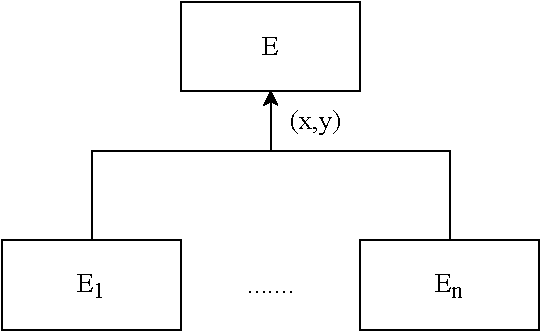
\includegraphics[width=.5\textwidth]{img/generalizzazione_sintassi.pdf}
		\end{figure}
		\newpage
		
		
		\item \textcolor{Green4}{\emph{Si illustri il concetto/costrutto di \textbf{identificatore} nel modello Entità-Relazione.}}
		
		\textbf{Semantica}. Gli identificatori descrivono i concetti (attributi/entità) dello schema che consentono di identificare in maniera univoca le occorrenze delle entità. Devono essere specificati per ogni entità e non possono apparire all'interno di relazioni. Un identificatore può essere:
		\begin{itemize}
			\item Interno, ovvero viene scelto un attributo dell'entità;
			\item Esterno, viene scelto un identificatore di un'altra identità;
		\end{itemize}
		È possibile utilizzare sia identificatori interni ed esterni insieme.\newline
		\textbf{Sintassi grafica}. Un esempio è l'entità \dquotes{Studente} che possiede come identificatore la \dquotes{Matricola} poiché unica. La sintassi grafica:
		\begin{figure}[!htp]
			\centering
			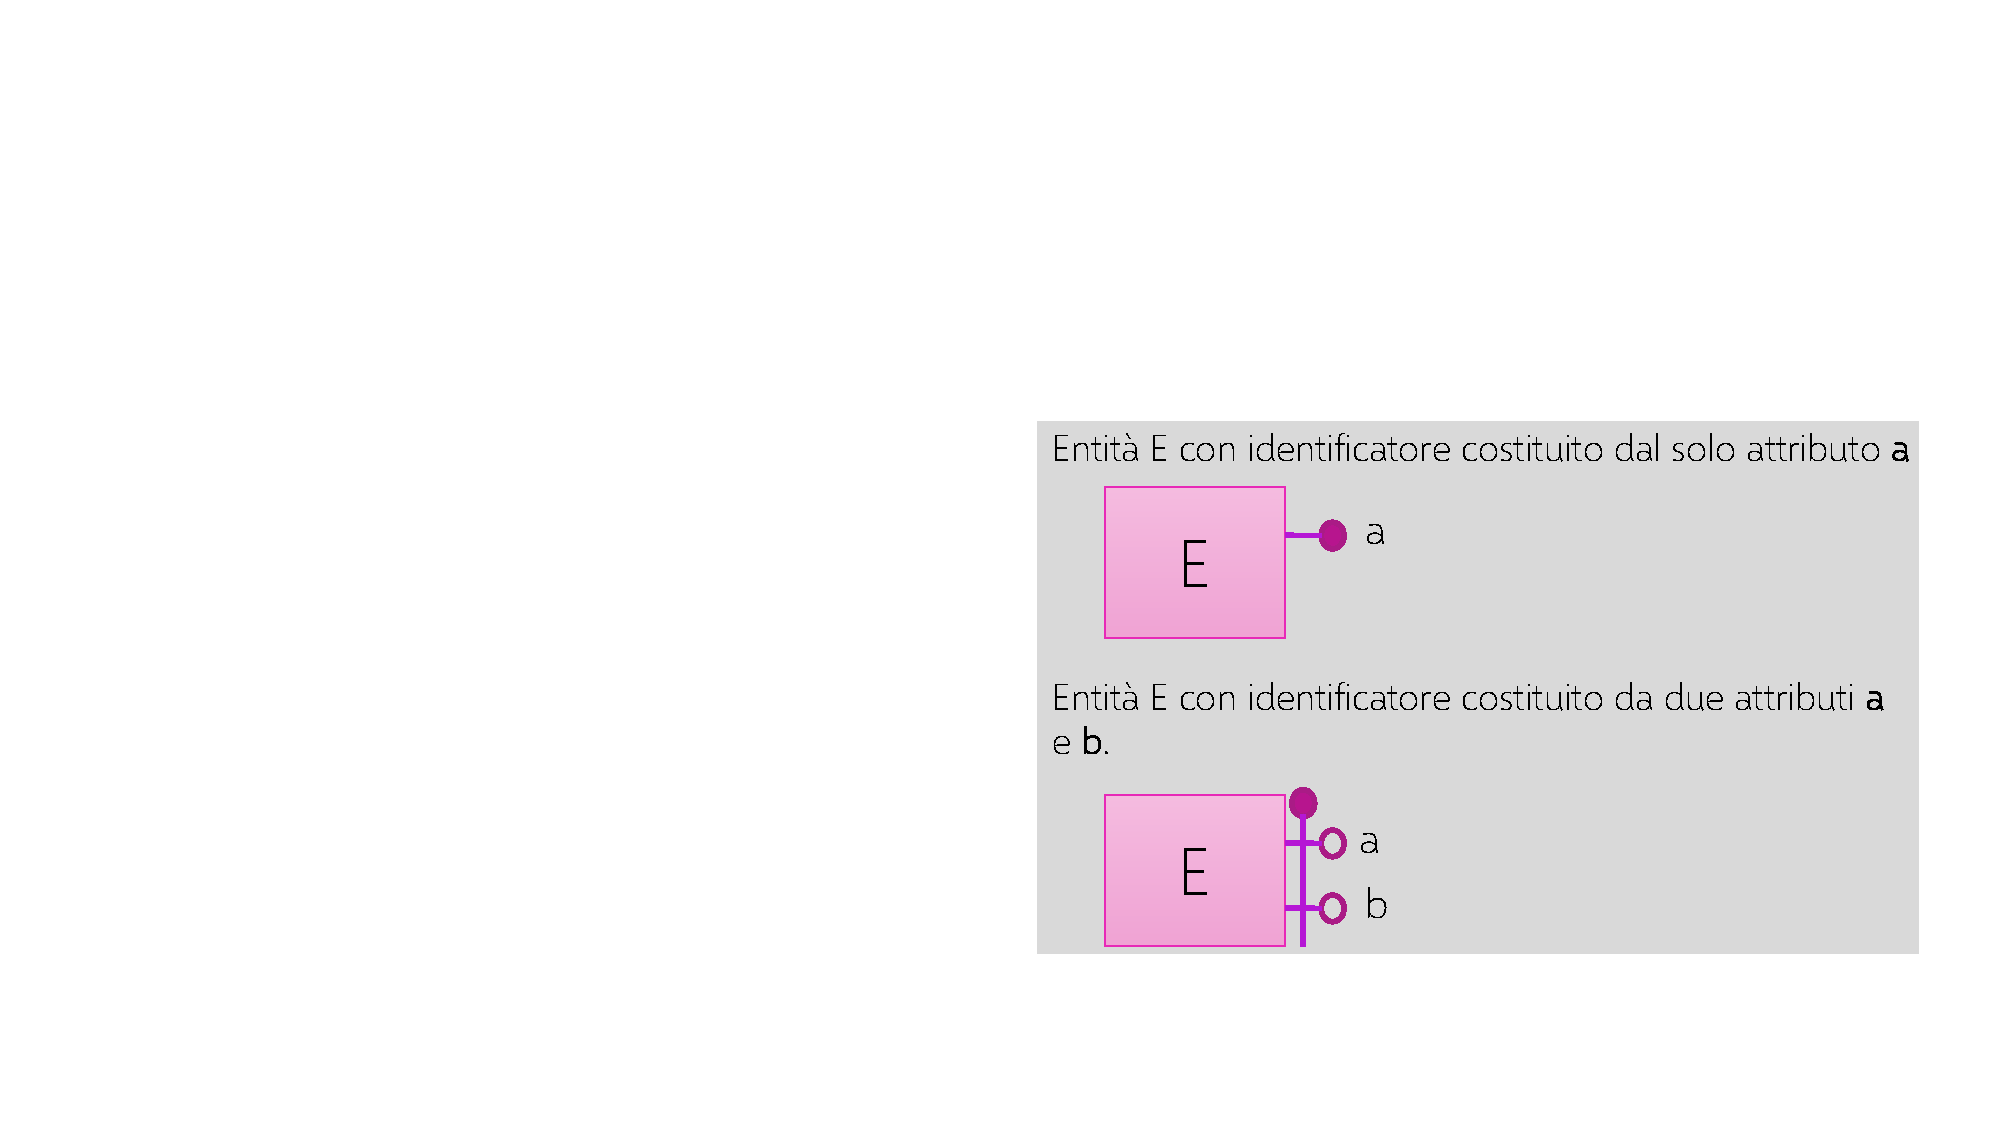
\includegraphics[width=.6\textwidth]{img/identificatore_def.pdf}
		\end{figure}
		
		
		\item \textcolor{Green4}{\emph{Si illustri il concetto/costrutto di \textbf{superchiave} nel modello Entità-Relazione.}}
		
		\textbf{Semantica}. Una superchiave è un'insieme di attributi che non contiene tuple duplicate al suo interno. Una superchiave è una chiave prima se e solo se è una superchiave minimale. Invece, una chiave primaria è sempre superchiave (non viceversa!).\newline
		\textbf{Sintassi grafica}. Non esiste una sintassi grafica poiché è un concetto, ma un esempio:
		\begin{figure}[!htp]
			\centering
			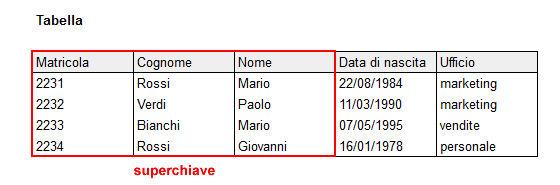
\includegraphics[width=\textwidth]{img/superchiave.png}
		\end{figure}
		
		\noindent
		Nessuna tupla si ripete, quindi \dquotes{Matricola, Cognome, Nome} è una superchiave valida. Non è minimale poiché esiste \dquotes{Matricola} che è chiave primaria e superchiave minimale.
		\newpage
		
		
		\item \textcolor{Green4}{\emph{Si illustri il concetto/costrutto di \textbf{attributo} nel modello Entità-Relazione.}}
		
		\textbf{Semantica}. Gli attributi descrivono le proprietà elementari di entità o relazioni che sono di interesse ai fini dell'applicazione. Ogni attributo ha un suo dominio e quindi può essere visto come una funzione che ha come dominio le istanze dell'entità/relazione e come codominio l'insieme dei valori ammissibili:
		\begin{equation*}
			f_{a} : I\left(E\right) \rightarrow D
		\end{equation*}
		Dove $a$ è un attributo dell'entità $E$, $I\left(E\right)$ è l'insieme delle istanze di $E$ e $D$ è l'insieme dei valori ammissibili.\newline
		\textbf{Sintassi grafica}. Un esempio di attributo è \dquotes{Cognome}, \dquotes{Stipendio} ed \dquotes{Età} dell'entità \dquotes{Impiegato}. La sintassi grafica è la seguente:
		\begin{figure}[!htp]
			\centering
			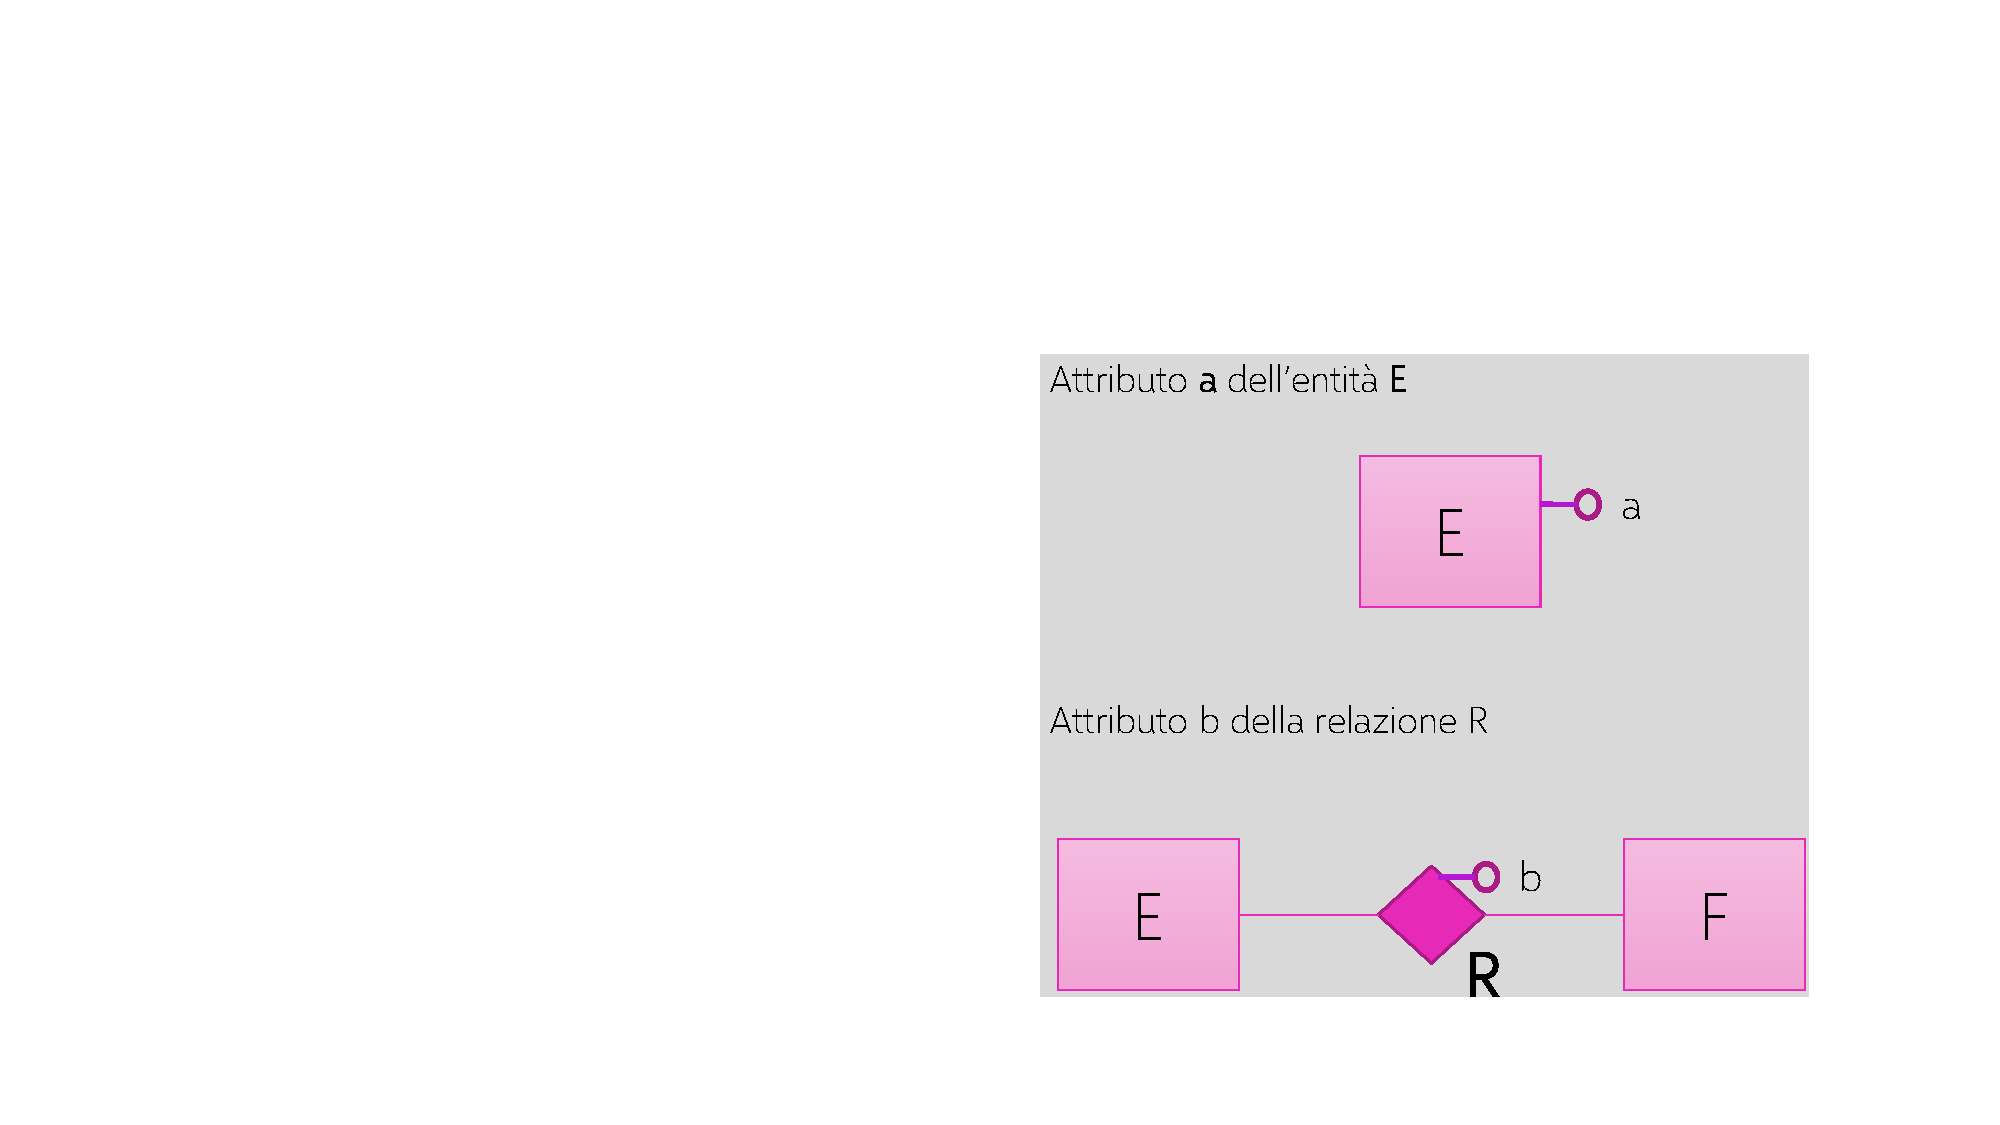
\includegraphics[width=.5\textwidth]{img/attributo_def.pdf}
		\end{figure}
		
		\noindent
		\textbf{Istanza}. L'istanza si ottiene tramite una funzione che data un'istanza dell'entità $E$ (o relazione $R$), restituisce l'attributo $a$:
		\begin{equation*}
			\text{valore di} \: a \: \text{su} \: e = f_{a}\left(e\right)
		\end{equation*}
	\end{enumerate}\newpage
	
	\section{Esercizi terzo parziale}
	
	\subsection[$\mathrm{B^{+}\text{-}tree}$]{$\boldsymbol{\mathrm{B^{+}\text{-}tree}}$}
	
	\subsubsection{Esercizio 1}
	
	Costruire un $\mathrm{B}^{+}$-tree di $\text{fan-out} = 5$ con i seguenti nodi foglia: $\left(A,B,C,D\right)$, $\left(F,G,M,N\right)$, $\left(O,P\right)$, $\left(S,T\right)$, $\left(W,Z\right)$. I vincoli di riempimento sono:
	\begin{itemize}
		\item $2 \le \text{\#chiavi} \le 4$
		
		\item $3 \le \text{\#puntatori} \le 5$
	\end{itemize}
	Dopodiché, inserire il valore chiave H nel $\mathrm{B}^{+}$-tree ottenuto precedentemente. Infine, l'esercizio si conclude eseguendo una rimozione del valore chiave Z ottenuto precedentemente.\newline
	
	\noindent
	\textcolor{Green4}{\textbf{\emph{\underline{Soluzione}}}}\newline
	
	\noindent
	Il primo passo è costruire i vari livelli dei nodi foglia:
	\begin{figure}[!htp]
		\centering
		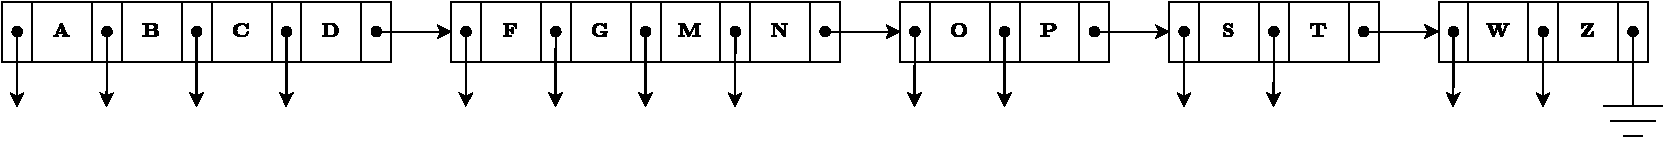
\includegraphics[width=\textwidth]{img/b+-tree.pdf}
	\end{figure}
	
	\noindent
	Adesso è necessario costruire tutti i puntatori richiesti. Fan-out è uguale a 5 quindi viene costruito un nodo intermedio con 5 puntatori e si collegano tutti i nodi:
	\begin{figure}[!htp]
		\centering
		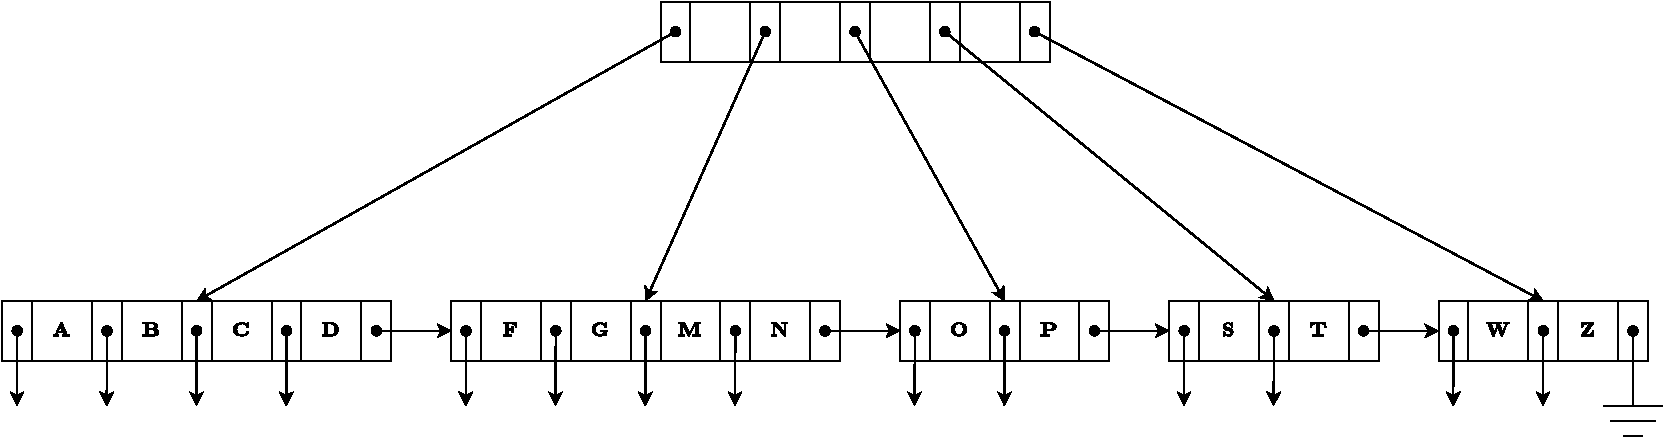
\includegraphics[width=\textwidth]{img/b+-tree-1.pdf}
	\end{figure}
	
	\noindent
	Adesso si aggiungono le lettere che devono essere raggiunte dopo aver visitato ogni nodo:
	\begin{figure}[!htp]
		\centering
		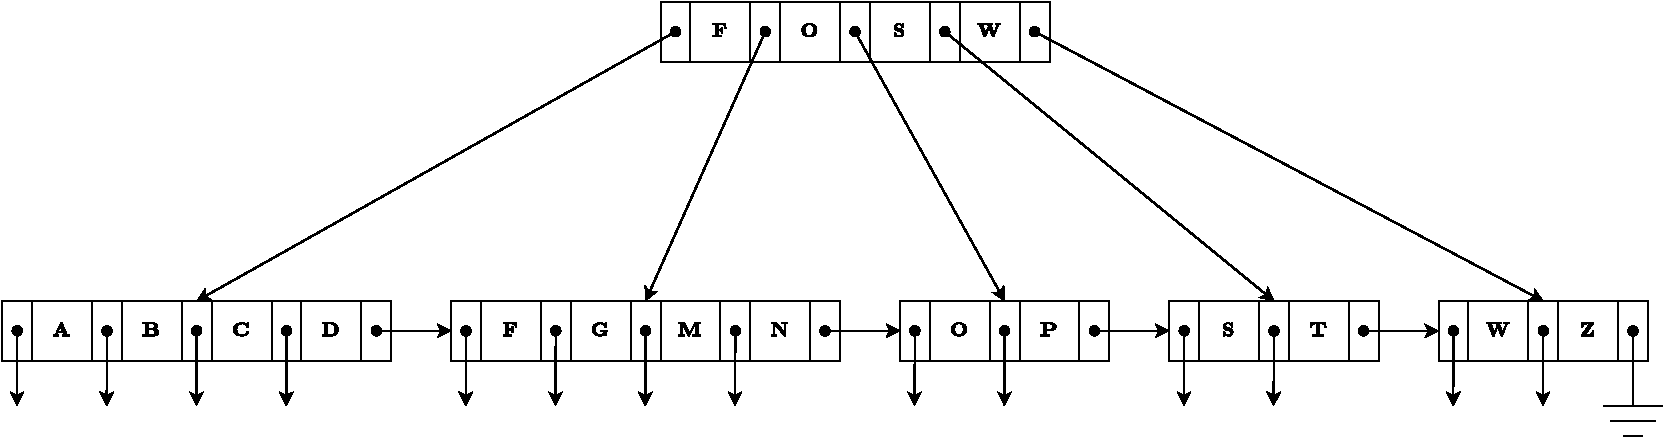
\includegraphics[width=\textwidth]{img/b+-tree-2.pdf}
	\end{figure}\newpage
	
	\noindent
	Per inserire il valore chiave è necessario avere a disposizione una posizione libera. Tuttavia, questo non è possibile, per cui viene applicato uno split. Viene divisa la radice contenente $\left(F,G,M,N\right)$ così da inserire la chiave H tra la G e la M:
	\begin{figure}[!htp]
		\centering
		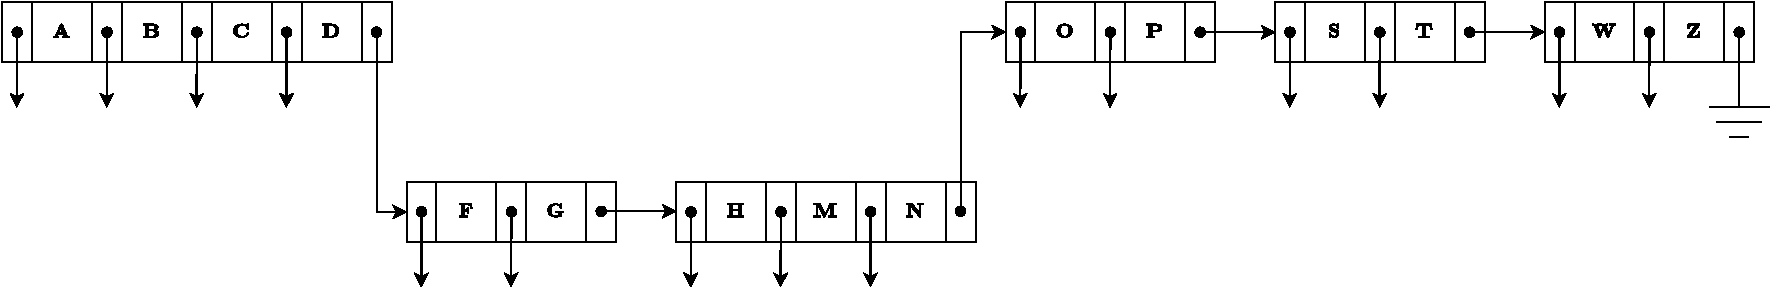
\includegraphics[width=\textwidth]{img/b+-tree-3.pdf}
	\end{figure}
	
	\noindent
	A questo punto è necessario riadattare il nodo radice che attualmente punta ad un nodo errato (attenzione c'è un errore, il nodo V in realtà è il nodo W):
	\begin{figure}[!htp]
		\centering
		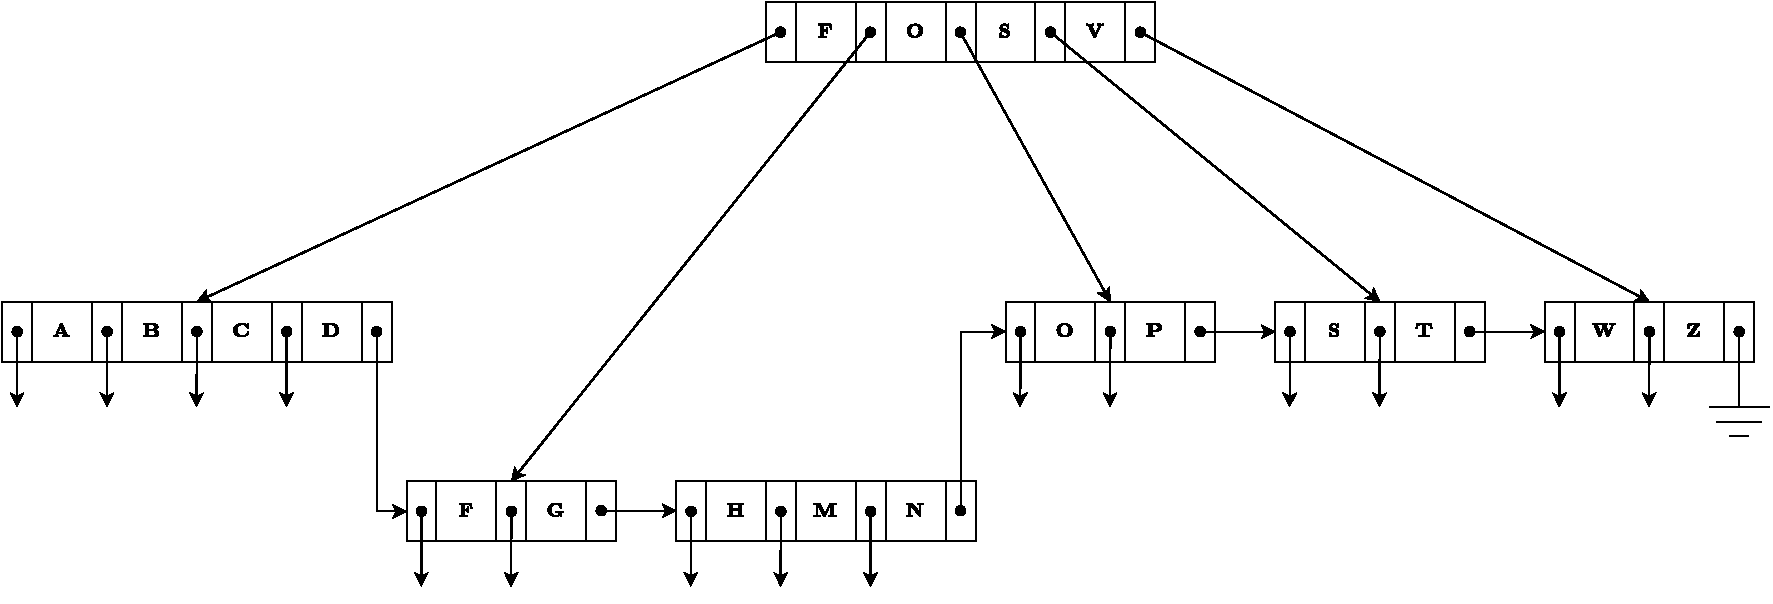
\includegraphics[width=\textwidth]{img/b+-tree-4.pdf}
	\end{figure}
	
	\noindent
	Per farlo, è necessario eseguire una divisione anche nel nodo radice aggiustando i valori delle chiavi (attenzione c'è un errore, il nodo V in realtà è il nodo W):
	\begin{figure}[!htp]
		\centering
		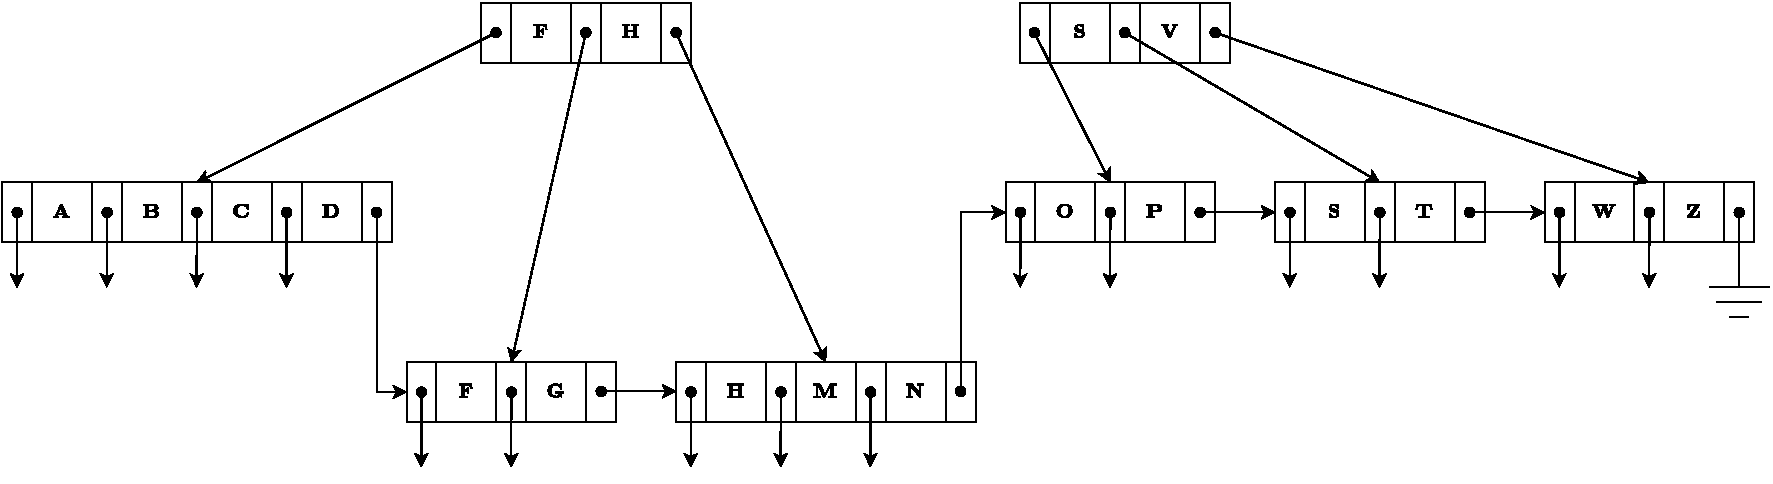
\includegraphics[width=\textwidth]{img/b+-tree-5.pdf}
	\end{figure}\newpage
	
	\noindent
	E infine, collegare i due nodi divisi con un nodo di congiunzione. Inoltre, quest'ultimo viene riempito con un valore chiave (attenzione c'è un errore, il nodo V in realtà è il nodo W):
	\begin{figure}[!htp]
		\centering
		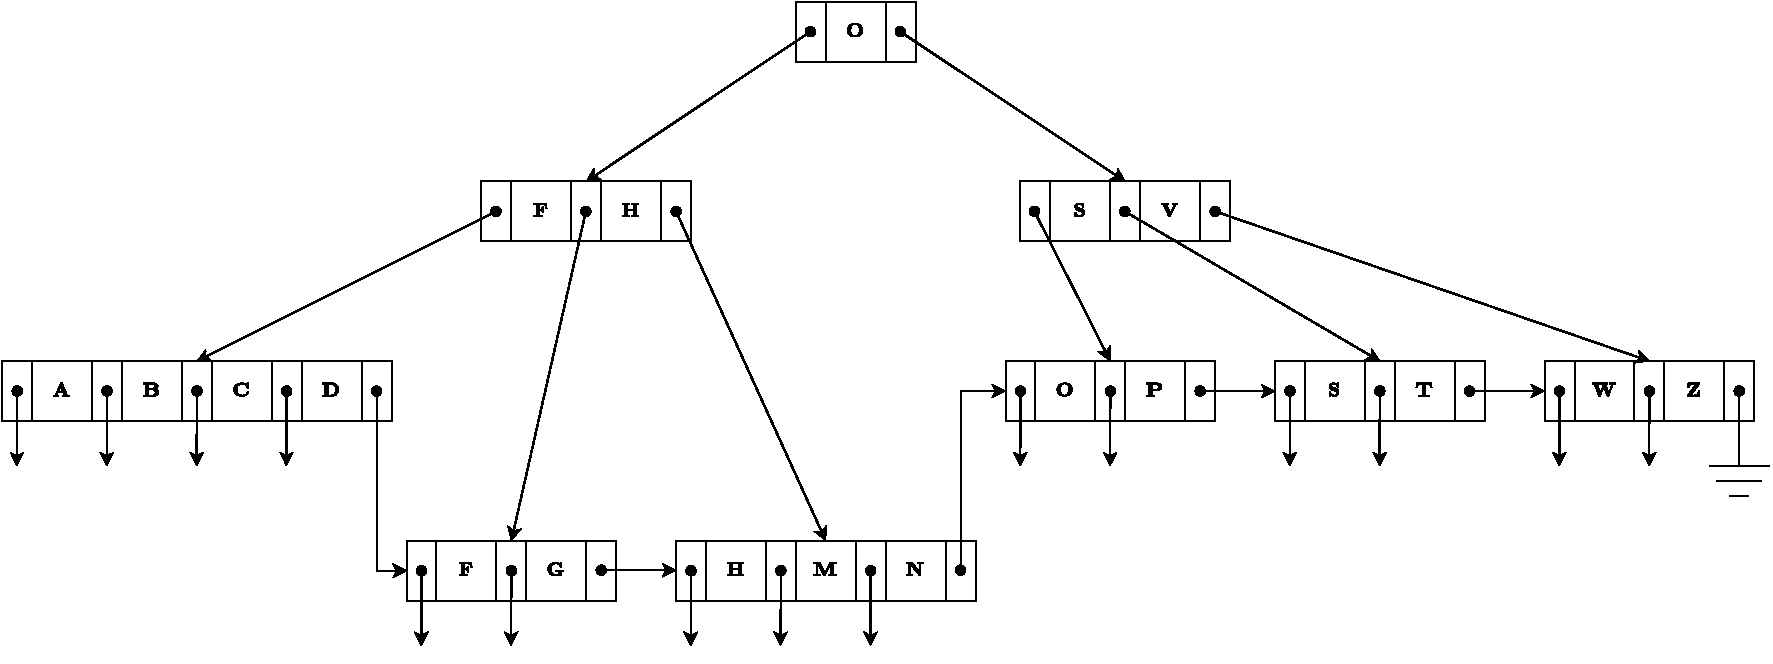
\includegraphics[width=\textwidth]{img/b+-tree-6.pdf}
	\end{figure}
	
	\noindent
	La rimozione della chiave Z comporta che l'ultimo nodo abbia come chiave solo il valore W. Questo comporta un'irregolarità poiché il numero minimo di ogni chiave in ogni nodo deve essere minimo di due e massimo di quattro. Per cui è necessario effettuare un merge:
	\begin{figure}[!htp]
		\centering
		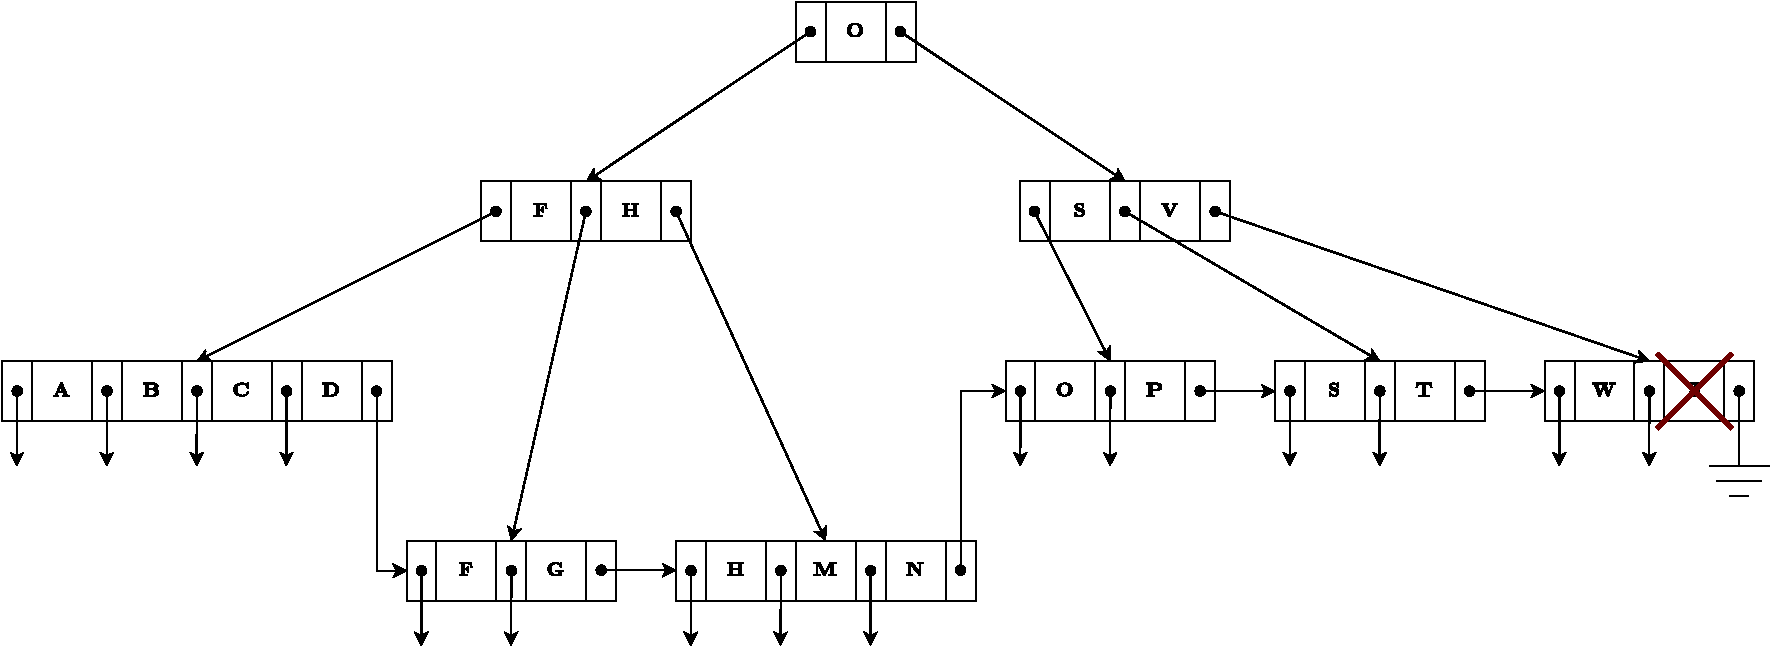
\includegraphics[width=\textwidth]{img/b+-tree-7.pdf}
		\caption*{Eliminazione della chiave Z.}
	\end{figure}
	
	\begin{figure}[!htp]
		\centering
		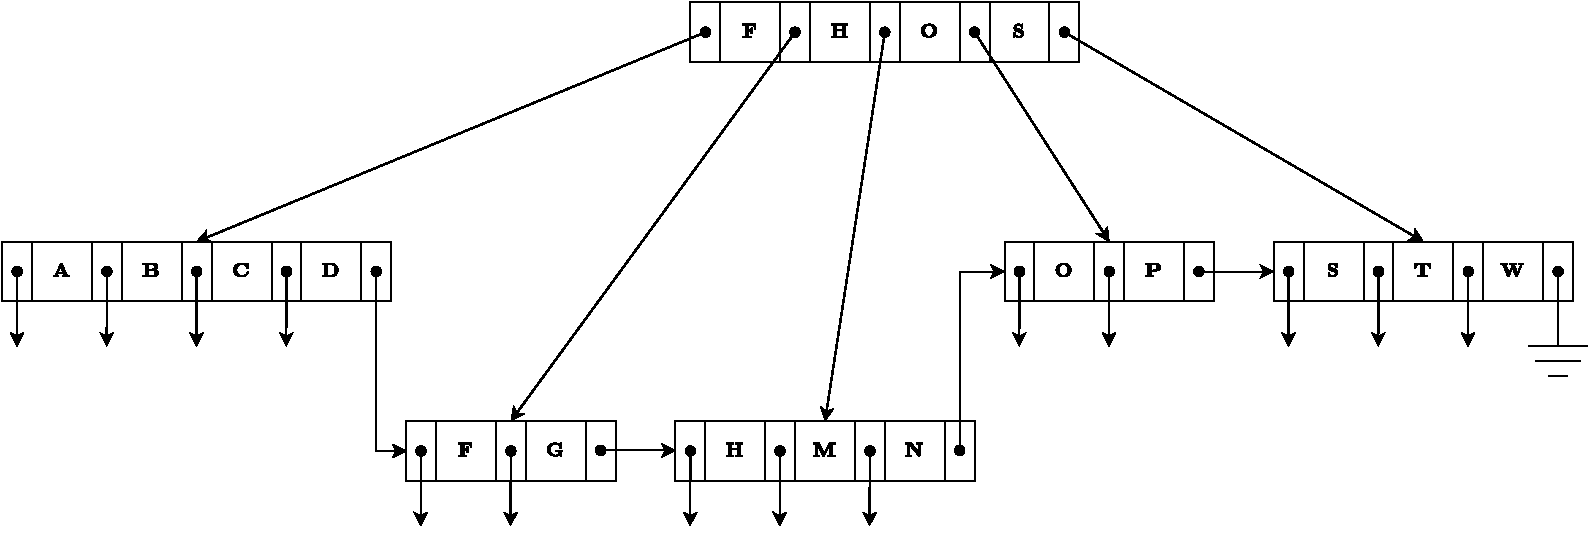
\includegraphics[width=\textwidth]{img/b+-tree-8.pdf}
		\caption*{Merge degli ultimi due nodi.}
	\end{figure}\newpage
	
	\subsection{Verificare che uno schedule sia VSR (View-serializzabilità)}
	
	\subsubsection{Esercizio 1 - Perdita di aggiornamento}
	
	Date due transazioni $T_{1}$ e $T_{2}$ di seguito descritte:
	\begin{equation*}
		\begin{array}{lll}
			T_{1} &:& r_{1}\left(x\right) \: w_{1}\left(x\right) \\
			T_{2} &:& r_{2}\left(x\right) \: w_{2}\left(x\right)
		\end{array}
	\end{equation*}
	Lo schedule che rappresenta l'anomalia è il seguente:
	\begin{equation*}
		S_{PA} = r_{1}\left(x\right) \: r_{2}\left(x\right) \: w_{2}\left(x\right) \: w_{1}\left(x\right)
	\end{equation*}
	Per verificare che uno schedule sia VSR o meno, è necessario caratterizzare $S_{PA}$ calcolando l'insieme delle relazioni LeggeDa e l'insieme delle ScrittureFinali.\newline
	
	\noindent
	Quindi, per l'insieme LeggeDa viene cercato per ogni operazione di lettura, una precedente scrittura sulla stessa risorsa fatta da un'altra transazione. In questo caso, l'insieme è vuoto poiché nessuna risorsa scrive prime di una lettura.\newline
	
	\noindent
	Invece, per l'insieme ScrittureFinali, per ogni risorsa indicata nello schedule si specifica l'ultima scrittura eseguita. In questo caso, l'unica risorsa è $x$ e l'ultima scrittura è $w_{1}\left(x\right)$.\newline
	
	\noindent
	Quindi, gli insiemi sono composti da:
	\begin{equation*}
		\begin{array}{rll}
			\text{LeggeDa}\left(S_{PA}\right) &=& \emptyset \\
			\text{ScrittureFinali}\left(S_{PA}\right) &=& \left\{w_{1}\left(x\right)\right\}
		\end{array}
	\end{equation*}
	Adesso si generano tutti i possibili schedule seriali che eseguono le due transazioni. Essi si ottengono generando le possibili permutazioni dell'insieme di transazioni che partecipano allo schedule. In questo caso, date solo due transazioni $T_{1}$ e $T_{2}$, le possibili combinazioni sono:
	\begin{equation*}
		\begin{array}{lllll}
			S_{1} &=& T_{1} \: T_{2} &=& r_{1}\left(x\right) \: w_{1}\left(x\right) \: r_{2}\left(x\right) \: w_{2}\left(x\right) \\
			S_{2} &=& T_{2} \: T_{1} &=& r_{2}\left(x\right) \: w_{2}\left(x\right) \: r_{1}\left(x\right) \: w_{1}\left(x\right) \\
		\end{array}
	\end{equation*}
	Adesso, si verifica che almeno uno dei due schedule seriali è view-equivalente a $S_{PA}$.\newpage
	
	\noindent
	Verifica partendo dallo schedule $S_{1}$:
	\begin{enumerate}
		\item Creazione dell'insieme LeggeDa$\left(S_{1}\right)$. Data la sequenza:
		\begin{equation*}
			S_{1} = r_{1}\left(x\right) \: w_{1}\left(x\right) \: r_{2}\left(x\right) \: w_{2}\left(x\right)
		\end{equation*}
		L'unica scrittura che precede una lettura è $w_{1}\left(x\right)$. Quindi, l'insieme è composto dalla scrittura che avviene prima della lettura e da quest'ultima:
		\begin{equation*}
			\text{LeggeDa}\left(S_{1}\right) = \left\{\left(r_{2}\left(x\right), w_{1}\left(x\right)\right)\right\}
		\end{equation*}
		
		\item Creazione dell'insieme ScrittureFinali$\left(S_{1}\right)$. Data la sequenza:
		\begin{equation*}
			S_{1} = r_{1}\left(x\right) \: w_{1}\left(x\right) \: r_{2}\left(x\right) \: w_{2}\left(x\right)
		\end{equation*}
		L'unica risorsa $x$ ha come ultima scrittura $w_{2}\left(x\right)$, quindi l'insieme è composto da:
		\begin{equation*}
			\text{ScrittureFinali}\left(S_{1}\right) = \left\{w_{2}\left(x\right)\right\}
		\end{equation*}
		
		\item Si esegue il confronto degli insiemi ottenuti da $S_{1}$ e dagli insiemi ottenuti da $S_{PA}$:
		\begin{equation*}
			\begin{array}{lll}
				\text{LeggeDa}\left(S_{PA}\right)	&=& \emptyset \\
				\text{LeggeDa}\left(S_{1}\right)	&=& \left\{\left(r_{2}\left(x\right), w_{1}\left(x\right)\right)\right\} \\
				\text{ScrittureFinali}\left(S_{PA}\right)	&=& \left\{w_{1}\left(x\right)\right\} \\
				\text{ScrittureFinali}\left(S_{1}\right)	&=& \left\{w_{2}\left(x\right)\right\}
			\end{array}
		\end{equation*}
		Come è evidente, nessuno dei due insiemi è equivalente:
		\begin{equation*}
			\begin{array}{lll}
				\text{LeggeDa}\left(S_{PA}\right)	&\cancel{\equiv}& \text{LeggeDa}\left(S_{1}\right) \\
				\text{ScrittureFinali}\left(S_{PA}\right)	&\cancel{\equiv}& \text{ScrittureFinali}\left(S_{1}\right)
			\end{array}
		\end{equation*}
		Quindi, è possibile concludere che $S_{PA}$ non è view-equivalente a $S_{1}$.
	\end{enumerate}\newpage
	
	\noindent
	Verifica partendo dallo schedule $S_{2}$:
	\begin{enumerate}
		\item Creazione dell'insieme LeggeDa$\left(S_{2}\right)$. Data la sequenza:
		\begin{equation*}
			S_{2} = r_{2}\left(x\right) \: w_{2}\left(x\right) \: r_{1}\left(x\right) \: w_{1}\left(x\right)
		\end{equation*}
		L'unica scrittura che precede una lettura è $w_{2}\left(x\right)$. Quindi, l'insieme è composto dalla scrittura che avviene prima della lettura e da quest'ultima:
		\begin{equation*}
			\text{LeggeDa}\left(S_{2}\right) = \left\{\left(r_{1}\left(x\right), w_{2}\left(x\right)\right)\right\}
		\end{equation*}
		
		\item Creazione dell'insieme ScrittureFinali$\left(S_{2}\right)$. Data la sequenza:
		\begin{equation*}
			S_{2} = r_{2}\left(x\right) \: w_{2}\left(x\right) \: r_{1}\left(x\right) \: w_{1}\left(x\right)
		\end{equation*}
		L'unica risorsa $x$ ha come ultima scrittura $w_{2}\left(x\right)$, quindi l'insieme è composto da:
		\begin{equation*}
			\text{ScrittureFinali}\left(S_{2}\right) = \left\{w_{1}\left(x\right)\right\}
		\end{equation*}
		
		\item Si esegue il confronto degli insiemi ottenuti da $S_{1}$ e dagli insiemi ottenuti da $S_{PA}$:
		\begin{equation*}
			\begin{array}{lll}
				\text{LeggeDa}\left(S_{PA}\right)	&=& \emptyset \\
				\text{LeggeDa}\left(S_{1}\right)	&=& \left\{\left(r_{1}\left(x\right), w_{2}\left(x\right)\right)\right\} \\
				\text{ScrittureFinali}\left(S_{PA}\right)	&=& \left\{w_{1}\left(x\right)\right\} \\
				\text{ScrittureFinali}\left(S_{1}\right)	&=& \left\{w_{1}\left(x\right)\right\}
			\end{array}
		\end{equation*}
		Come è evidente, soltanto uno dei due insiemi è equivalente:
		\begin{equation*}
			\begin{array}{lll}
				\text{LeggeDa}\left(S_{PA}\right)	&\cancel{\equiv}& \text{LeggeDa}\left(S_{1}\right) \\
				\text{ScrittureFinali}\left(S_{PA}\right)	&\equiv& \text{ScrittureFinali}\left(S_{1}\right)
			\end{array}
		\end{equation*}
		Quindi, è possibile concludere che $S_{PA}$ non è view-equivalente a $S_{1}$ poiché entrambi gli insiemi non sono equivalenti.
	\end{enumerate}
	L'esercizio si conclude qua. Nessuna combinazione è view-equivalente allo schedule di partenza $S_{PA}$. Quindi, si conclude affermando che $S_{PA}$ non è VSR.\newpage
	
	\subsubsection{Esercizio 2 - Lettura inconsistente}
	
	Date due transazioni $T_{1}$ e $T_{2}$ di seguito descritte:
	\begin{equation*}
		\begin{array}{lll}
			T_{1} &:& r_{1}\left(x\right) \: r_{1}'\left(x\right) \\
			T_{2} &:& r_{2}\left(x\right) \: w_{2}\left(x\right)
		\end{array}
	\end{equation*}
	Lo schedule che rappresenta l'anomalia è il seguente:
	\begin{equation*}
		S_{LI} = r_{1}\left(x\right) \: r_{2}\left(x\right) \: w_{2}\left(x\right) \: r_{1}'\left(x\right)
	\end{equation*}
	Per verificare che uno schedule sia VSR o meno, è necessario caratterizzare $S_{LI}$ calcolando l'insieme delle relazioni LeggeDa e l'insieme delle ScrittureFinali.\newline
	
	\noindent
	Quindi, per l'insieme LeggeDa viene cercato per ogni operazione di lettura, una precedente scrittura sulla stessa risorsa fatta da un'altra transazione. In questo caso, l'insieme è composto da $w_{2}\left(x\right)$ perché precede $r_{1}'\left(x\right)$.\newline
	
	\noindent
	Invece, per l'insieme ScrittureFinali, per ogni risorsa indicata nello schedule si specifica l'ultima scrittura eseguita. In questo caso, l'unica risorsa è $x$ e l'ultima scrittura è $w_{2}\left(x\right)$.\newline
	
	\noindent
	Quindi, gli insiemi sono composti da:
	\begin{equation*}
		\begin{array}{rll}
			\text{LeggeDa}\left(S_{LI}\right) &=& \left\{\left(r_{1}'\left(x\right), w_{2}\left(x\right)\right)\right\} \\
			\text{ScrittureFinali}\left(S_{LI}\right) &=& \left\{w_{2}\left(x\right)\right\}
		\end{array}
	\end{equation*}
	Adesso si generano tutti i possibili schedule seriali che eseguono le due transazioni. Essi si ottengono generando le possibili permutazioni dell'insieme di transazioni che partecipano allo schedule. In questo caso, date solo due transazioni $T_{1}$ e $T_{2}$, le possibili combinazioni sono:
	\begin{equation*}
		\begin{array}{lllll}
			S_{1} &=& T_{1} \: T_{2} &=& r_{1}\left(x\right) \: r_{1}'\left(x\right) \: r_{2}\left(x\right) \: w_{2}\left(x\right) \\
			S_{2} &=& T_{2} \: T_{1} &=& r_{2}\left(x\right) \: w_{2}\left(x\right) \: r_{1}\left(x\right) \: r_{1}'\left(x\right) \\
		\end{array}
	\end{equation*}
	Adesso, si verifica che almeno uno dei due schedule seriali è view-equivalente a $S_{LI}$.\newpage
	
	\noindent
	Verifica partendo dallo schedule $S_{1}$:
	\begin{enumerate}
		\item Creazione dell'insieme LeggeDa$\left(S_{1}\right)$. Data la sequenza:
		\begin{equation*}
			S_{1} = r_{1}\left(x\right) \: r_{1}'\left(x\right) \: r_{2}\left(x\right) \: w_{2}\left(x\right)
		\end{equation*}
		L'unica scrittura che precede una lettura è $w_{1}\left(x\right)$. Quindi, l'insieme è composto dalla scrittura che avviene prima della lettura e da quest'ultima:
		\begin{equation*}
			\text{LeggeDa}\left(S_{1}\right) = \emptyset
		\end{equation*}
		
		\item Creazione dell'insieme ScrittureFinali$\left(S_{1}\right)$. Data la sequenza:
		\begin{equation*}
			S_{1} = r_{1}\left(x\right) \: r_{1}'\left(x\right) \: r_{2}\left(x\right) \: w_{2}\left(x\right)
		\end{equation*}
		L'unica risorsa $x$ ha come ultima scrittura $w_{2}\left(x\right)$, quindi l'insieme è composto da:
		\begin{equation*}
			\text{ScrittureFinali}\left(S_{1}\right) = \left\{w_{2}\left(x\right)\right\}
		\end{equation*}
		
		\item Si esegue il confronto degli insiemi ottenuti da $S_{1}$ e dagli insiemi ottenuti da $S_{LI}$:
		\begin{equation*}
			\begin{array}{lll}
				\text{LeggeDa}\left(S_{LI}\right)	&=& \left\{\left(r_{1}'\left(x\right), w_{2}\left(x\right)\right)\right\} \\
				\text{LeggeDa}\left(S_{1}\right)	&=& \emptyset \\
				\text{ScrittureFinali}\left(S_{LI}\right)	&=& \left\{w_{2}\left(x\right)\right\} \\
				\text{ScrittureFinali}\left(S_{1}\right)	&=& \left\{w_{2}\left(x\right)\right\}
			\end{array}
		\end{equation*}
		Come è evidente, soltanto uno dei due insiemi è equivalente:
		\begin{equation*}
			\begin{array}{lll}
				\text{LeggeDa}\left(S_{LI}\right)	&\cancel{\equiv}& \text{LeggeDa}\left(S_{1}\right) \\
				\text{ScrittureFinali}\left(S_{LI}\right)	&\equiv& \text{ScrittureFinali}\left(S_{1}\right)
			\end{array}
		\end{equation*}
		Quindi, è possibile concludere che $S_{LI}$ non è view-equivalente a $S_{1}$.
	\end{enumerate}\newpage
	
	\noindent
	Verifica partendo dallo schedule $S_{2}$:
	\begin{enumerate}
		\item Creazione dell'insieme LeggeDa$\left(S_{2}\right)$. Data la sequenza:
		\begin{equation*}
			S_{2} = r_{2}\left(x\right) \: w_{2}\left(x\right) \: r_{1}\left(x\right) \: r_{1}'\left(x\right)
		\end{equation*}
		L'unica scrittura che precede due letture è $w_{2}\left(x\right)$. Quindi, l'insieme è composto dalla scrittura che avviene con due letture:
		\begin{equation*}
			\text{LeggeDa}\left(S_{2}\right) = \left\{\left(r_{1}'\left(x\right), w_{2}\left(x\right)\right), \left(r_{1}\left(x\right), w_{2}\left(x\right)\right)\right\}
		\end{equation*}
		
		\item Creazione dell'insieme ScrittureFinali$\left(S_{2}\right)$. Data la sequenza:
		\begin{equation*}
			S_{2} = r_{2}\left(x\right) \: w_{2}\left(x\right) \: r_{1}\left(x\right) \: r_{1}'\left(x\right)
		\end{equation*}
		L'unica risorsa $x$ ha come ultima scrittura $w_{2}\left(x\right)$, quindi l'insieme è composto da:
		\begin{equation*}
			\text{ScrittureFinali}\left(S_{2}\right) = \left\{w_{2}\left(x\right)\right\}
		\end{equation*}
		
		\item Si esegue il confronto degli insiemi ottenuti da $S_{1}$ e dagli insiemi ottenuti da $S_{PA}$:
		\begin{equation*}
			\begin{array}{lll}
				\text{LeggeDa}\left(S_{LI}\right)	&=& \left\{\left(r_{1}'\left(x\right), w_{2}\left(x\right)\right)\right\} \\
				\text{LeggeDa}\left(S_{2}\right)	&=& \left\{\left(r_{1}'\left(x\right), w_{2}\left(x\right)\right), \left(r_{1}\left(x\right), w_{2}\left(x\right)\right)\right\} \\
				\text{ScrittureFinali}\left(S_{LI}\right)	&=& \left\{w_{2}\left(x\right)\right\} \\
				\text{ScrittureFinali}\left(S_{2}\right)	&=& \left\{w_{2}\left(x\right)\right\}
			\end{array}
		\end{equation*}
		Come è evidente, soltanto uno dei due insiemi è equivalente:
		\begin{equation*}
			\begin{array}{lll}
				\text{LeggeDa}\left(S_{PA}\right)	&\cancel{\equiv}& \text{LeggeDa}\left(S_{1}\right) \\
				\text{ScrittureFinali}\left(S_{PA}\right)	&\equiv& \text{ScrittureFinali}\left(S_{1}\right)
			\end{array}
		\end{equation*}
		Quindi, è possibile concludere che $S_{LI}$ non è view-equivalente a $S_{2}$ poiché entrambi gli insiemi non sono equivalenti.
	\end{enumerate}
	L'esercizio si conclude qua. Nessuna combinazione è view-equivalente allo schedule di partenza $S_{LI}$. Quindi, si conclude affermando che $S_{LI}$ non è VSR.\newpage
	
	\subsubsection{Sintesi dell'algoritmo}
	
	In sintesi l'algoritmo per capire se uno schedule è VSR:
	\begin{enumerate}
		\item Si tiene bene in considerazione lo schedule che rappresenta l'anomalia, ovvero quello che viene dato;
		
		\item Si compongono i due insiemi:
		\begin{enumerate}
			\item Creazione insieme LeggeDa cercando per ogni operazione di lettura ($r_{i}\left(\text{risorsa}\right)$) una precedente operazione di scrittura sulla stessa risorsa fatta da un'altra transazione. Nel caso in cui si trovi, si aggiunge all'insieme la scrittura incriminata e la relativa lettura;
			
			\item Creazione insieme ScrittureFinali cercando per ogni risorsa indicata nello schedule l'ultima scrittura eseguita.
		\end{enumerate}
		
		\item Date le varie transazioni, si creano tutti i possibili schedule creando così una lista;
		
		\item Si verifica che almeno uno schedule della lista sia view-equivalente allo schedule dato al punto 1. Per farlo si esegue questo piccolo algoritmo:
		\begin{enumerate}
			\item Creazione dell'insieme LeggeDa (vedi punto 2.a);
			
			\item Creazione dell'insieme ScrittureFinali (vedi punto 2.b);
			
			\item Confronto degli insiemi creati precedente con quelli creati per lo schedule dato al punto 1. Se non sono uguali tutti uguali, allora lo schedule creato tramite combinazione non è equivalente allo schedule dato al punto 1. Altrimenti, è possibile affermare di aver trovato una combinazione view-equivalente.
		\end{enumerate}
		
		\item Al termine della creazione degli insiemi e dei vari confronti, se esiste almeno una combinazione che è view-equivalente allo schedule del punto 1, allora è possibile affermare che lo schedule di partenza è VSR.
	\end{enumerate}\newpage
	
	\subsection{Verificare che uno schedule sia CSR}
	
	\subsubsection{Esercizio 1 - Perdita di aggiornamento}
	
	Date due transizioni $T_{1}$ e $T_{2}$:
	\begin{equation*}
		\begin{array}{lll}
			T_{1} &:& r_{1}\left(x\right) \: w_{1}\left(x\right) \\
			T_{2} &:& r_{2}\left(x\right) \: w_{2}\left(x\right)
		\end{array}
	\end{equation*}
	Lo schedule che rappresenta l'anomalia è il seguente:
	\begin{equation*}
		S_{PA} = r_{1}\left(x\right) \: r_{2}\left(x\right) \: w_{2}\left(x\right) \: w_{1}\left(x\right)
	\end{equation*}
	Per verificare CSR è necessario caratterizzare $S_{PA}$ calcolando l'insieme dei conflitti. Si ricorda che due azioni sono in conflitto se operano sullo stesso oggetto e se almeno una di esse è in scrittura (quindi le combinazioni: $rw, wr, ww$). Quindi, si calcola l'insieme dei conflitti di $S_{PA}$:
	\begin{enumerate}
		\item $\textcolor{Red3}{r_{1}\left(x\right)} \: r_{2}\left(x\right) \: \textcolor{Red3}{w_{2}\left(x\right)} \: w_{1}\left(x\right)$
		
		\item $r_{1}\left(x\right) \: \textcolor{Red3}{r_{2}\left(x\right)} \: w_{2}\left(x\right) \: \textcolor{Red3}{w_{1}\left(x\right)}$
		
		\item $r_{1}\left(x\right) \: r_{2}\left(x\right) \: \textcolor{Red3}{w_{2}\left(x\right)} \: \textcolor{Red3}{w_{1}\left(x\right)}$
	\end{enumerate}
	L'insieme è quindi così costituito:
	\begin{equation*}
		\text{Conflitti}\left(S_{PA}\right) = \left\{\left(r_{1}\left(x\right), w_{2}\left(x\right)\right), \left(r_{2}\left(x\right), w_{1}\left(x\right)\right), \left(w_{2}\left(x\right), w_{1}\left(x\right)\right)\right\}
	\end{equation*}
	Si costruisce il grafo nel seguente modo. Si rappresentano tanti nodi quanti sono le transazioni e ogni arco (orientato) viene tracciato da $t_{i}$ a $t_{j}$ se vengono rispettate due condizioni: se c'è almeno un conflitto fra un'azione $a_{i}$ e un'azione $a_{j}$ tale che $a_{i}$ precede $a_{j}$. Quindi:
	\begin{figure}[!htp]
		\centering
		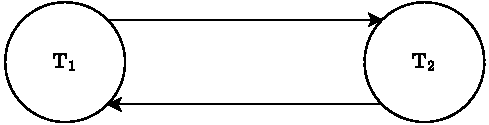
\includegraphics[width=.55\textwidth]{img/CSR-1.pdf}
	\end{figure}
	
	\noindent
	Se il grafo è aciclico allora $S_{PA}$ è CSR. In questo caso, il grafo non è aciclico ma ciclico, per cui $S_{PA}$ non è CSR.\newpage
	
	\subsubsection{Esercizio 2 - Lettura inconsistente}
	
	Date due transizioni $T_{1}$ e $T_{2}$:
	\begin{equation*}
		\begin{array}{lll}
			T_{1} &:& r_{1}\left(x\right) \: r_{1}'\left(x\right) \\
			T_{2} &:& r_{2}\left(x\right) \: w_{2}\left(x\right)
		\end{array}
	\end{equation*}
	Lo schedule che rappresenta l'anomalia è il seguente:
	\begin{equation*}
		S_{LI} = r_{1}\left(x\right) \: r_{2}\left(x\right) \: w_{2}\left(x\right) \: r_{1}'\left(x\right)
	\end{equation*}
	Per verificare CSR è necessario caratterizzare $S_{LI}$ calcolando l'insieme dei conflitti. Si ricorda che due azioni sono in conflitto se operano sullo stesso oggetto e se almeno una di esse è in scrittura (quindi le combinazioni: $rw, wr, ww$). Quindi, si calcola l'insieme dei conflitti di $S_{LI}$:
	\begin{enumerate}
		\item $\textcolor{Red3}{r_{1}\left(x\right)} \: r_{2}\left(x\right) \: \textcolor{Red3}{w_{2}\left(x\right)} \: r_{1}'\left(x\right)$
		
		\item $r_{1}\left(x\right) \: r_{2}\left(x\right) \: \textcolor{Red3}{w_{2}\left(x\right)} \: \textcolor{Red3}{r_{1}'\left(x\right)}$
	\end{enumerate}
	L'insieme è quindi così costituito:
	\begin{equation*}
		\text{Conflitti}\left(S_{LI}\right) = \left\{\left(r_{1}\left(x\right), w_{2}\left(x\right)\right), \left(w_{2}\left(x\right), r_{1}'\left(x\right)\right)\right\}
	\end{equation*}
	Si costruisce il grafo nel seguente modo. Si rappresentano tanti nodi quanti sono le transazioni e ogni arco (orientato) viene tracciato da $t_{i}$ a $t_{j}$ se vengono rispettate due condizioni: se c'è almeno un conflitto fra un'azione $a_{i}$ e un'azione $a_{j}$ tale che $a_{i}$ precede $a_{j}$. Quindi:
	\begin{figure}[!htp]
		\centering
		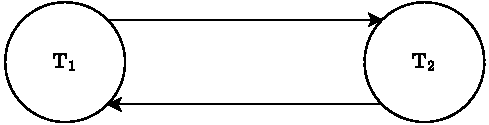
\includegraphics[width=.55\textwidth]{img/CSR-1.pdf}
	\end{figure}
	
	\noindent
	Se il grafo è aciclico allora $S_{LI}$ è CSR. In questo caso, il grafo non è aciclico ma ciclico, per cui $S_{LI}$ non è CSR.
	
	\longline
	
	\subsubsection{Sintesi dell'algoritmo}
	
	In sintesi l'algoritmo per capire se uno schedule è CSR:
	\begin{enumerate}
		\item Si calcola l'insieme dei conflitti. Un conflitto si manifesta quando due azioni operano sullo stesso oggetto e quando almeno una di esse è in scrittura. Quindi, le combinazioni che possono esserci sono: $rw, wr, ww$;
		
		\item Si costruire il grafo dall'insieme dei conflitti. I nodi rappresentano le transizioni e gli archi si disegnano solo se due azioni non riguardano la stessa transizione.
	\end{enumerate}\newpage
	
	\subsection{Verificare che uno schedule sia NonSR, VSR e/o CSR}
	
	\subsubsection{Testo esercizio}
	
	Classificare i seguenti schedule (come: NonSR, VSR, CSR); nel caso uno schedule sia VSR oppure CSR, indicare tutti gli schedule seriali a esso equivalenti.
	\begin{enumerate}
		\item $S_{1} = r_{1}\left(x\right) \: w_{1}\left(x\right) \: r_{2}\left(z\right) \: r_{1}\left(y\right) \: w_{1}\left(y\right) \: r_{2}\left(x\right) \: w_{2}\left(x\right) \: w_{2}\left(z\right)$
		
		\item $S_{2} = r_{1}\left(x\right) \: w_{1}\left(x\right) \: w_{3}\left(x\right) \: r_{2}\left(y\right) \: r_{3}\left(y\right) \: w_{3}\left(y\right) \: w_{1}\left(y\right) \: r_{2}\left(x\right)$
		
		\item $S_{3} = r_{1}\left(x\right) \: r_{2}\left(x\right) \: w_{2}\left(x\right) \: r_{3}\left(x\right) \: r_{4}\left(z\right) \: w_{1}\left(x\right) \: w_{3}\left(y\right) \: w_{3}\left(x\right) \: w_{1}\left(y\right) \: w_{5}\left(x\right) \: w_{1}\left(z\right) \: w_{5}\left(y\right) \: r_{5}\left(z\right)$
		
		\item $S_{4} = r_{1}\left(x\right) \: r_{3}\left(y\right) \: w_{1}\left(y\right) \: w_{4}\left(x\right) \: w_{1}\left(t\right) \: w_{5}\left(x\right) \: r_{2}\left(z\right) \: r_{3}\left(z\right) \: w_{2}\left(z\right) \: w_{5}\left(z\right) \: r_{4}\left(t\right) \: r_{5}\left(t\right)$
	\end{enumerate}
	
	\longline
	
	\subsubsection{Schedule 1}
	
	Dato il seguente schedule:
	\begin{equation*}
		S_{1} = r_{1}\left(x\right) \: w_{1}\left(x\right) \: r_{2}\left(z\right) \: r_{1}\left(y\right) \: w_{1}\left(y\right) \: r_{2}\left(x\right) \: w_{2}\left(x\right) \: w_{2}\left(z\right)
	\end{equation*}
	Le transizioni sono:
	\begin{equation*}
		\begin{array}{lll}
			T_{1} &:& r_{1}\left(x\right) \: w_{1}\left(x\right) \: r_{1}\left(y\right) \: w_{1}\left(y\right) \\
			T_{2} &:& r_{2}\left(z\right) \: r_{2}\left(x\right) \: w_{2}\left(x\right) \: w_{2}\left(z\right)
		\end{array}
	\end{equation*}
	Si verifica se è CSR. Quindi, si crea l'insieme dei conflitti:
	\begin{enumerate}
		\item $\textcolor{Red3}{r_{1}\left(x\right)} \: w_{1}\left(x\right) \: r_{2}\left(z\right) \: r_{1}\left(y\right) \: w_{1}\left(y\right) \: r_{2}\left(x\right) \: \textcolor{Red3}{w_{2}\left(x\right)} \: w_{2}\left(z\right)$
		
		\item $r_{1}\left(x\right) \: \textcolor{Red3}{w_{1}\left(x\right)} \: r_{2}\left(z\right) \: r_{1}\left(y\right) \: w_{1}\left(y\right) \: \textcolor{Red3}{r_{2}\left(x\right)} \: w_{2}\left(x\right) \: w_{2}\left(z\right)$
		
		\item $r_{1}\left(x\right) \: \textcolor{Red3}{w_{1}\left(x\right)} \: r_{2}\left(z\right) \: r_{1}\left(y\right) \: w_{1}\left(y\right) \: r_{2}\left(x\right) \: \textcolor{Red3}{w_{2}\left(x\right)} \: w_{2}\left(z\right)$
	\end{enumerate}
	Quindi l'insieme è:
	\begin{equation*}
		\text{Conflitti}\left(S_{1}\right) = \left\{\left(r_{1}\left(x\right) \: w_{2}\left(x\right)\right), \left(w_{1}\left(x\right) \: r_{2}\left(x\right)\right), \left(w_{1}\left(x\right) \: w_{2}\left(x\right)\right)\right\}
	\end{equation*}
	Si costruisce il grafo:
	\begin{figure}[!htp]
		\centering
		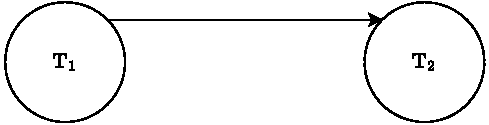
\includegraphics[width=.55\textwidth]{img/NoSR-VSR-CSR-1.pdf}
	\end{figure}
	
	\noindent
	Il ciclo è aciclico quindi è $S_{1}$ è CSR. Dato che CSR $\subset$ VSR, allora $S_{1}$ è anche VSR.\newpage
	
	\subsubsection{Schedule 2}
	
	Dato il seguente schedule:
	\begin{equation*}
		S_{2} = r_{1}\left(x\right) \: w_{1}\left(x\right) \: w_{3}\left(x\right) \: r_{2}\left(y\right) \: r_{3}\left(y\right) \: w_{3}\left(y\right) \: w_{1}\left(y\right) \: r_{2}\left(x\right)
	\end{equation*}
	Le transazioni sono:
	\begin{equation*}
		\begin{array}{lll}
			T_{1} &:& r_{1}\left(x\right) \: w_{1}\left(x\right) \: w_{1}\left(y\right) \\
			T_{2} &:& r_{2}\left(y\right) \: r_{2}\left(x\right) \\
			T_{3} &:& w_{3}\left(x\right) \: r_{3}\left(y\right) \: w_{3}\left(y\right)
		\end{array}
	\end{equation*}
	Si verifica se è VSR. Si inizia analizzando l'insieme $S_{2}$:
	\begin{equation*}
		\begin{array}{lll}
			\text{LeggeDa}\left(S_{2}\right) 			&=& \left\{\left(r_{2}\left(x\right), w_{3}\left(x\right)\right)\right\} \\
			\text{ScrittureFinali}\left(S_{2}\right) 	&=& \left\{w_{3}\left(x\right), w_{1}\left(y\right)\right\}
		\end{array}
	\end{equation*}
	Dato che è impossibile provare tutte le combinazioni (3 transazioni e quindi $3! = 6$), si fanno alcune considerazioni. Per esempio, dato che nelle LeggeDa si deve mantenere l'ordine $\left(r_{2}\left(x\right), w_{3}\left(x\right)\right)$, e sapendo che $r_{2}$ appartiene a $T_{2}$ e $w_{3}$ a $T_{3}$, si può concludere che $T_{3}$ deve per forza precedere $T_{2}$. Quindi, le combinazioni si riducono a:
	\begin{itemize}
		\item $T_{1} \: T_{3} \: T_{2}$
		
		\item $T_{3} \: T_{1} \: T_{2}$
		
		\item $T_{3} \: T_{2} \: T_{1}$
	\end{itemize}
	Tuttavia, se $T_{3}$ anticipa $T_{2}$, tutte le combinazioni avranno come insieme LeggeDa \underline{almeno} i due valori:
	\begin{equation*}
		\text{LeggeDa}\left(S_{2}\right) = \left\{\left(r_{2}\left(x\right), w_{3}\left(x\right)\right), \left(r_{2}\left(y\right) \: w_{3}\left(y\right)\right)\right\}
	\end{equation*}
	Quindi, è possibile concludere che nessuna combinazione ha un insieme LeggeDa equivalente al LeggeDa di $S_{2}$. È possibile concludere che $S_{2}$ non è VSR.\newpage
	
	\subsubsection{Schedule 3}
	
	Dato il seguente schedule:
	\begin{equation*}
		S_{3} = r_{1}\left(x\right) \: r_{2}\left(x\right) \: w_{2}\left(x\right) \: r_{3}\left(x\right) \: r_{4}\left(z\right) \: w_{1}\left(x\right) \: w_{3}\left(y\right) \: w_{3}\left(x\right) \: w_{1}\left(y\right) \: w_{5}\left(x\right) \: w_{1}\left(z\right) \: w_{5}\left(y\right) \: r_{5}\left(z\right)
	\end{equation*}
	
	\subsubsection{Schedule 4}
	
	\subsubsection{Verifica}
	
	\subsection{Ottimizzazione e stima di costo}
	
	\subsubsection{Esercizio 1}
	
	\subsection{XML}
	
	\subsubsection{Esercizio 1}
	
	\subsubsection{Esercizio 2}
	
	\section{Esami terzo parziale}
	
	\subsection{Terzo parziale - 06/2015}
	
	\subsection{Terzo parziale - 07/06/2016}
	
	\subsection{Terzo parziale - 21/04/2022}
	
	\subsection{Terzo parziale - 22/04/2022}
	
	\subsection{Terzo parziale - 10/06/2022}
\end{document}